\chapter{Public Transport}
\label{ch:pt}
% ##################################################################################################################

\hfill \textbf{Authors:} Marcel Rieser, Andreas Neumann, Johan W. Joubert, Sergio Arturo Ordóñez

\begin{center} 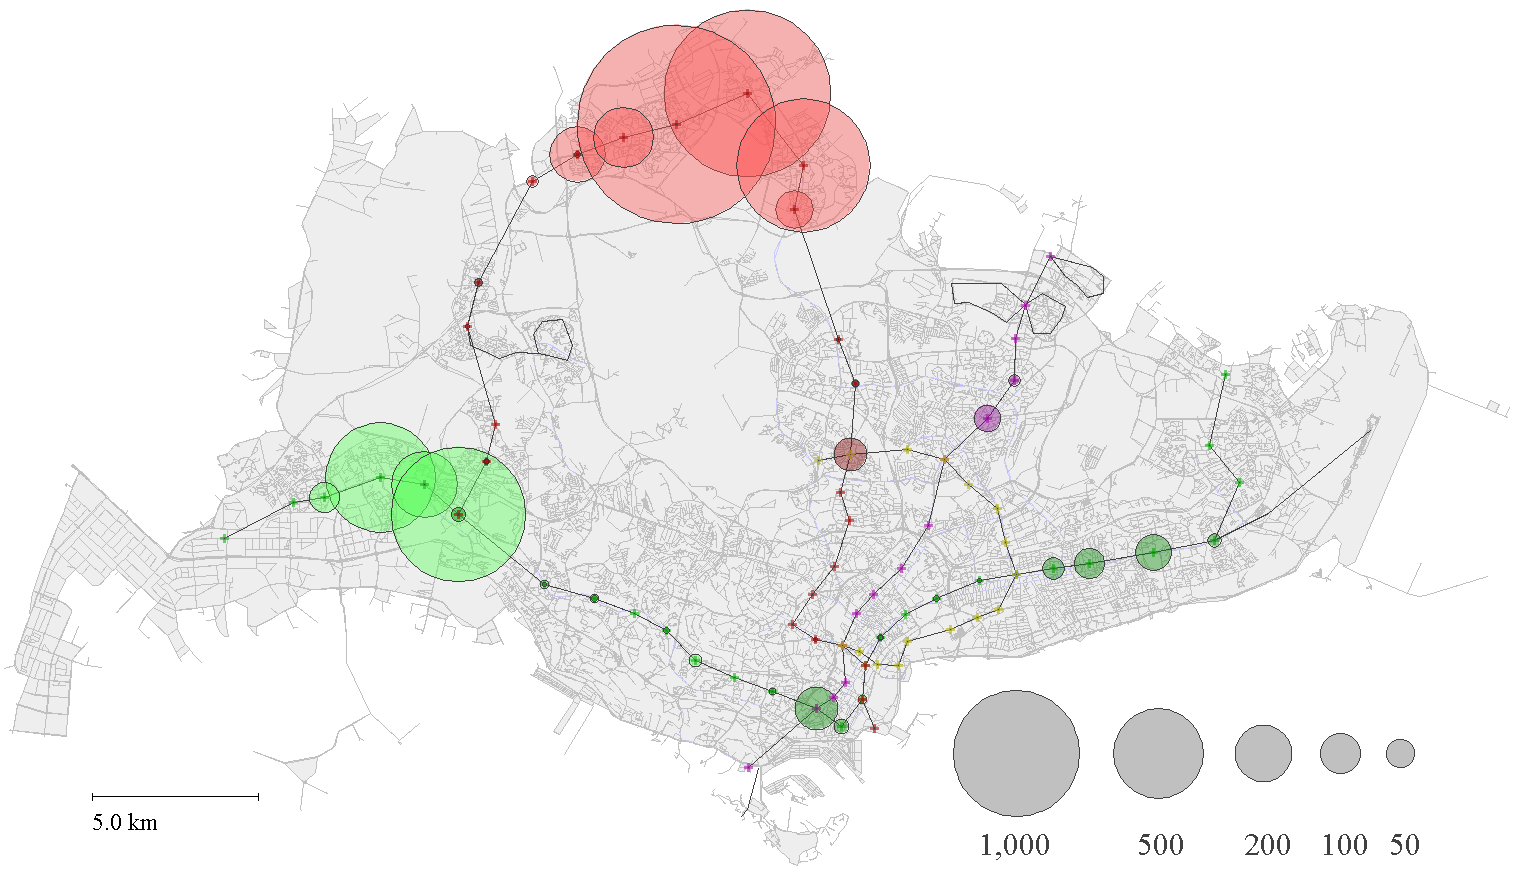
\includegraphics[width=0.25\textwidth, angle=0]{extending/figures/ebr/Backwards.png} \end{center}

\createStandardInformationBasic{{\url{http://matsim.org/javadoc} $\to$ core $\to$ pt package}}{The module is invoked by enabling it in the configuration.}{\lstinline{transit} section(s) of the config file.
}{\citet{Rieser2010,Neumann2014PhD}}
\ah{GTFS2TransitSchedule is also in there!}

% ##################################################################################################################
\section{Modeling Public Transport with MATSim}
\subsection{Introduction}
Public transport---or \emph{transit} as it is sometimes called---plays
an important role in many transport planning measures, even if they only target
non-transit modes in the first place. By making other modes more or less
attractive (\eg by providing higher capacity with additional lanes, allowing
higher speeds, or charging money by setting up road pricing for an area), people
might reconsider their mode choice and switch to public transport (\emph{pt})
from other modes, or vice versa. Such changes can also occur when the transit
infrastructure is changed: additional bus lines, changed tram routes with
different stops served, altered headways, all have an influence whether
people tend to us a specific line, or public transport in general. Around 2007,
it was thus a central point to extend \gls{matsim} to support simulation of other
modes besides private car traffic, and especially to simulate public transport
in detail.

In a first step, \gls{matsim} was extended in such a way that modes other than
\emph{car} would be \gls{teleported}, that is agents would be removed at one location
and placed at a later point of time---corresponding to the estimated travel time---at
their destination location, where they could commence their next activity.
Together with a simple mode-choice module, randomly replacing all the
transport modes in all legs of a plan, and a simple travel time estimation for
modes different than \emph{car}, first case studies resulting in modal share
changes were performed using \gls{matsim}
\citep{RieserGretherNagel2008modeChoiceCalculations,
GretherEtAl2009SimpleModeChoiceIPL}. This \gls{teleportation} mode is now available by
default in \gls{matsim} and still a very good fallback to get a \gls{multimodal} scenario
up and running with as few data as possible.

In a second step, \gls{qsim} was extended to support the detailed simulation of
public transport vehicles that serve stops along fixed routes with a given schedule
\citep{Rieser2010}.
The next section will describe the required data and resulting features for this
detailed public transport simulation in more detail.

% ============================================================================================
\subsection{Data Model and Simulation Features}
\gls{matsim} supports modeling public transport in a high level of detail: transit
vehicles run along the defined routes of transit lines, picking up
and dropping off passengers at stop locations, while taking care of the transit
vehicles' capacities and maximum speeds. The data used to simulate public
transport in \gls{matsim} can be split in three parts:
%
\begin{itemize}\styleItemize
\item Stop locations
\item Schedule, defining lines, routes and departures
\item Vehicles
\end{itemize}

This data is stored in two files, with the vehicles being defined in one
file and stop locations and schedule being defined in
another file.
Examples of such files can be seen in
Section~\ref{sec:inputdata:transitvehicles} and
Section~\ref{sec:inputdata:transitschedule}, respectively.

The data model is comparable to that of other public transport planning
software, but simplified in a few aspects. A line has typically two or more
routes: One route for each direction, and additional routes when vehicles start
(or end) their service somewhere in the middle of the full route when coming
from (or going to) a depot. Each transit route contains a network route,
specifying along which links in the network the transit vehicle drives along,
and a list of departures, providing the information at what time a vehicle
starts at the first stop of the route. A route also describes the ordered list
of stops that are being served along with timing information, when a vehicle
arrives or leaves a stop. This timing information is given as offsets only, to
be added to the departure time at the first stop. Each departure contains the
time at which a vehicle starts the route, and a reference to the vehicle that
runs this service. Because the timing information is part of the route, routes
with the same sequence of stops may exist, differing only in the time offsets.
This is often the case with bus lines that take traffic congestion and
longer waiting times at stops during rush hours into account in the schedule. 

Stop locations are described by their coordinates and an optional name, and must
be assigned to exactly one line of the network for the simulation. Thus, they
can be best compared to ``stop points'' in \gls{visum}. There is currently no logical
grouping of such stop locations to build a ``stop area''---a collection of
stops typically having the same name but, \eg on different arms of an intersection and
being served by different lines and where passengers can usually transfer
between).

Each vehicle belongs to one vehicle type. Such a vehicle type describes various
characteristics of a vehicle, like the seating and standing capacity (number of
passengers), its maximum speed, but also how many passengers can board or alight
a vehicle per second.

This data model already supports several advanced aspects of modeling public
transport, like having different travel speeds along routes during different
times of day (important for improved realism in the simulation), using vehicles
of different types on a route at different times of day (interesting for the
economic analysis of a schedule), and re-using transit vehicles for multiple
headways along one or different routes (allows the optimization of vehicle
deployment planning, or research the effects of delay-propagation).

With all this data set, the \gls{qsim} will simulate the movements of all
transit vehicles. The vehicles will start at the first stop of their route at the given
departure time, allow passengers to enter, and then drive along their route,
serving stops. At each stop, passengers can enter or leave the vehicle.
The simulation generates additional, transit-related events whenever a transit
vehicle arrives or departs at a stop, when passengers enter or leave a vehicle,
but also when a passenger cannot board a vehicle because the vehicle's capacity
limit is already reached. This allows for detailed analyses of the public transport
simulation performed by \gls{matsim}.

In order for passengers to use public transport in \gls{matsim}, they need to be able
to calculate a route using transit services. For this, \gls{matsim} includes a public
transport router which calculates the best route for arriving at the desired
destination with minimal cost, given a departure time. Costs are typically
defined as travel time only and a small penalty for changing lines, but other,
more complex cost functions could be used.

The routing algorithm is based on Dijkstra's shortest path algorithm
\citep{Dijkstra1959ShortestPath}, but modified in order to take
multiple possible transit stops around the start and the end coordinate
into account to find a route. Multiple start and end stops must be considered in
order to generate more realistic transit routes, as otherwise agents could
be forced to first travel into the wrong direction, or wait at an infrequently
served bus stop instead of going a bit further to a busy subway stop location.
By modifying the shortest path algorithm to work with multiple start and end
locations, a considerable performance gain was possible compared to the naive
implementation, calculating a route for each combination of start/end location
and then choosing the best out of it.

% -----------------------------------------------------------------------
\subsection{File formats}

\subsubsection{\lstinline|transitVehicles.xml|}
\label{sec:inputdata:transitvehicles}

%%\kai{convert to normal vehicles?}

%%\ah{copied from let's get started:}
%%\kai{vehicles.xml?  (without ``transit''?)} \kai{Andreas, fyi: I think we are leaning towards having separate containers vehicles.xml and transitVehicles.xml.  Not yet implemented.}

To simulate public transport in \gls{matsim}, two additional input files are necessary. One is \lstinline|transitVehicles.xml|, which describes the vehicles which serve the lines: are they big buses, small buses, trains or light rail vehicles, and describes how many passengers each vehicle can transport.

The description of public transport vehicles can be split into two parts: In a first part, vehicle types have to be described, specifying how many passengers such a vehicle can transport (Note that the term ``vehicle'' can refer to multiple vehicles in reality, \eg a train with several wagons should be specified as one long vehicle with a high number of seats). In the second part, actual vehicles have to be listed. Each vehicle has an identifier and is of a previously specified vehicle type. The following shows an example of a such a file, describing one vehicle type and two vehicles of that type. 

\begin{xml}
<?xml version="1.0" encoding="UTF-8"?> 
<vehicleDefinitions xmlns="http://www.matsim.org/files/dtd" 
       xmlns:xsi="http://www.w3.org/2001/XMLSchema-instance" 
       xsi:schemaLocation="http://www.matsim.org/files/dtd http://www.matsim.org/files/dtd/vehicleDefinitions_v1.0.xsd"> 
	<vehicleType id="1"> 
      <description>Small Train</description> 
      <capacity> 
         <seats persons="50"/> 
         <standingRoom persons="30"/> 
      </capacity> 
      <length meter="50.0"/> 
   </vehicleType> 
   <vehicle id="tr_1" type="1"/> 
   <vehicle id="tr_2" type="1"/> 
</vehicleDefinitions>
\end{xml}

% -----------------------------------------------------------------------
\subsubsection{\lstinline|transitSchedule.xml|}
\label{sec:inputdata:transitschedule}
The second file that is required to simulate public transport is \lstinline|transitSchedule.xml|, a rather complex file. It contains information about stop facilities (these can be bus stops, train stations or other stop locations) and transit services.

In the first part, the stop facilities need to be defined, giving each one a coordinate, an identifier and a reference to a link in the network. The stop can only be served by vehicles driving on that specified link. Optionally, it is possible to specify a name for the stop and if other vehicles are blocked when a transit vehicle is waiting at a stop. This last attribute is useful to model \eg the difference of bus stops, where one bus stop has a bay, while at another stop, the bus has to stop on the actual road.

After the stop facilities, the transit lines, their routes and schedules are described. This is a hierarchical data structure: Each line can have one or more routes, each route has a route profile, a network route and a list of departures. The following listing represents an example of a minimalistic but complete transit schedule.
%
\begin{xml}
<?xml version="1.0" encoding="UTF-8"?> 
<!DOCTYPE transitSchedule SYSTEM "http://www.matsim.org/files/dtd/transitSchedule_v1.dtd"> 
<transitSchedule> 
   <transitStops> 
      <stopFacility id="1" x="990.0"  y="0.0"   name="Adorf" 
           linkRefId="1" isBlocking="false"/> 
      <stopFacility id="2" x="1100.0" y="980.0" name="Beweiler" 
           linkRefId="2" isBlocking="true"/> 
      <stopFacility id="3" x="0.0"    y="10.0"  name="Cestadt" 
           linkRefId="3" isBlocking="false"/> 
   </transitStops> 
   <transitLine id="Blue Line"> 
      <transitRoute id="1"> 
         <description>Just a comment.</description> 
         <transportMode>bus</transportMode> 
         <routeProfile> 
            <stop refId="1" departureOffset="00:00:00"/> 
            <stop refId="2" arrivalOffset="00:02:30" departureOffset="00:03:00" 
                                                     awaitDeparture="true"/> 
            <stop refId="3" arrivalOffset="00:05:00" awaitDeparture="true"/> 
         </routeProfile> 
         <route> 
            <link refId="1"/> 
            <link refId="2"/> 
            <link refId="3"/> 
         </route> 
         <departures> 
            <departure id="1" departureTime="07:00:00" vehicleRefId="12"/> 
            <departure id="2" departureTime="07:05:00" vehicleRefId="23"/> 
            <departure id="3" departureTime="07:10:00" vehicleRefId="34"/> 
         </departures> 
      </transitRoute> 
   </transitLine> 
</transitSchedule>
\end{xml}

Each transit line must have a unique id. Each transit route has an id which must be unique within that one line, so the same route id can be used with different lines. The \lstinline|transportMode| describes on which links in the network the line runs (Actually, this is currently not yet enforced. It would be possible to let a bus run on train links in the simulation. It might be enforced in the future).

The \lstinline|routeProfile| describes the stops this route serves, while route itself describes the series of links in the network the transit vehicle's driver has to drive along (thus often referred to as network route. Note that the complete route, \ie all links the vehicle drives along, must be listed in the route, and not only the ones where stops are located. All the specified stops should occur along this route in the specified order. The time offsets given for each stop in the \lstinline|routeProfile| describe the relative time offset to an actual departure time. If a bus is to depart at 7\,am, and stop~2 has a \lstinline|departureOffset| 3\,minutes, this must be read that the bus is expected to depart at 7:03\,am at the specific stop. All stops in the route profile must have a departure offset defined, except the last one. All stops, except the first one, can optionally have an arrival offset defined. This is mostly useful for large trains that stop for several minutes at a station to help the routing algorithm to find connecting services at the correct time, namely the expected arrival time of the train.

As last part of the description of a transit route, the list of departures should be given. Each departure has an id, which must be unique within the route, and gives the departure time at the first stop of the specified route profile. In addition, the departure specifies with which vehicle the service should be run. This vehicle must be defined in the aforementioned list of transit vehicles. 

Because of its complexity, transit schedules often contain little mistakes that will return in an error when the simulation runs. Typical examples include that the network route is missing a link, or that the network route does not pass at all the defined stops in the right order. To make sure a schedule does not have any such issues before the simulation is started, a special validation routine is available:
%
\begin{lstlisting}
java -Xmx512m -cp /path/to/matsim.jar  
      org.matsim.pt.utils.TransitScheduleValidator  
      /path/to/transitSchedule.xml /path/to/network.xml
\end{lstlisting}
%
If run, this validator will print out a list of errors or warnings, if any are found, or show a message that the schedule appears to be valid.

% ============================================================================================
\subsection{Possible Improvements}
While the ability to simulate public transport was a big advance for \gls{matsim},
there are still several shortcomings that could see improvement:
%
\begin{itemize}\styleItemize
	\item The data model (and thus, the simulation) does not yet fully support some
	transit lines observed in the real world. Especially, circular lines without a
	defined start and end cannot be easily modeled yet. Also, some bus or
	train lines have stops where only boarding or alighting the vehicle is allowed,
	but not both (\eg overnight trains with sleeper cabins). At the moment, \gls{matsim}
	always allows boarding and alighting at stops, leading to agents \eg using a
	train with sleeper cabins only for a short trip, where in reality they would be
	denied boarding without a reservation for a longer trip.
	\item A stop location as seen by passengers in the real world is
	typically modeled as a number of stop facilities in \gls{matsim}, detailing the
	different locations where transit vehicles stop depending on their route and
	direction. For analysis purposes, one is often interested in aggregated values
	for such logical stop locations, and not for the individual stop facilities.
	Such a logical grouping is currently still missing in \gls{matsim} data format.
	\item Running simulations with a reduced sample of the population leads to
	artifacts when public transport is used. In a simulation with a sampled demand,
	network capacity is reduced accordingly to accommodate the fact that fewer
	private cars are on the road. But as still 100\,\% of public transport vehicles
	must run (albeit with reduced passenger capacity), the calibration becomes
	difficult. This should be solved in the future by not reducing the network
	capacity, but by giving each vehicle and agent a weight for how much it should
	count.
	\item The public transport router available and used by \gls{matsim} by default is
	strictly schedule based. It assumes, that the vehicles can keep up with the
	schedule and that enough passenger capacity is provided. In some regions, where
	transit offerings are notoriously delayed and overcrowded, \gls{matsim}'s router will
	consistently advise agents to use routes that will perform badly in the
	simulation. Additional feedback from the simulation back to the router, as it
	is already done in the private car router of \gls{matsim}, will be needed.
	\item Last but not least, the current router based on a modified shortest path
	algorithm of Dijkstra can become rather slow and memory-intensive for
	larger areas with exhaustive transit offerings. Improved algorithms to generate
	the routing graph, or different routing algorithms altogether (like the
	non-graph based Connection Scan Algorithm
	\citep{DibbeltEtAl_BonifaciEtAl_2013}) will have to be researched in the
	future.
\end{itemize}

% ============================================================================================
\subsection{Applications}
The public transport simulation has been used in a variety of applications of
\gls{matsim} world-wide. The following list highlights some of these applications,
pointing out specialties of them regarding the public transport simulation.

\begin{itemize}\styleItemize
	\item Berlin: The Berlin scenario (see Chapter~\ref{ch:berlinI}) was one of
	the first real applications using the public transport simulation in \gls{matsim}.
	The road and rail network as well as the full transit schedule was converted
	from a \gls{visum} model. It is yet one of the few known models where bus and tram
	lines share a common network with private car traffic, enabling full
	interaction between private and public vehicles like transit vehicles getting
	stuck in and delayed due to a traffic jam.
	%
	\item Switzerland: \gls{senozon} maintains a model of Switzerland, which contains the
	full time table of all buses, trams, trains, ships, and even cable cars in the
	Swiss alps. The schedule data is retrieved from the official time table,
	available in a machine-readable format called ``\gls{hafas} raw data format''.
	%
	\item Singapore: The model of Singapore (see Chapter~\ref{ch:singapore}) makes
	heavy use of public transport, and continually pushes the boundaries of what is
	currently possible to simulate. Due to the very large number of buses on
	Singapore's roads and the strong demand for it, a number of extensions had to
	be implemented in order to be able to realistically model pt in this context.
	%
	\item Minibus: The minibus contribution (see next Section~\ref{sec:paratransit}) 
	adds an optimization layer on top of the public
	transport functionality in \gls{matsim}, providing the functionality to automatically
	generate an optimized transit schedule for a certain region.
	%
	\item wagonsim: In the wagonsim contribution, %(see Section~\ref{sec:wagonsim})
	the public transport simulation was actually misused to simulate
	rail-bound freight traffic. While the simulation was still moving around
	transit vehicles and let passengers enter and leave such vehicles, the scenario
	was built in such a way that vehicles correspond to freight trains, and
	passengers correspond to the actual goods needing to be transported. Custom
	implementations of the transit driver logic replaces the definition of a
	vehicle's capacity by one that ensures that the trains the vehicles represent
	do not get too long or too heavy. The network was built in a way that changing
	vehicles at stops takes a minimum amount of time, corresponding to the time
	needed for switching wagons at freight terminals.
\end{itemize}

Besides the applications mentioned in the list above, many additional scenarios
make use of the public transport simulation in \gls{matsim} by now. But the list also
shows, that with some custom extensions and imagination, the public transport
functionality cannot only be used to ``just simulate public transport'', but be
used to solve complex problems previously being handled by operation research
groups.

% ##################################################################################################################
\section{Paratransit}
\label{sec:paratransit}
Paratransit is an informal, market-oriented, and self-organizing public transport system. 
Despite the great importance of this transport mode it is mainly unsubsidized and only relies on the collected fares. 
Paratransit systems can be categorized by route pattern and function, by organization of drivers, kind of stops, and fare type. 
Most case studies covered by the thesis of \citet[][]{Neumann_PhDThesis_2014} indicate that paratransit services are mainly 
organized as route associations operating 8-15\,seater vans on fixed routes. Most of the services run in direct competition to a
public transport system of a public transit authority. Such a service---minibuses with fixed routes but without fixed schedule---is often called a jitney service.
The minibus module of \gls{matsim} is based on those most common characteristics with the understanding that the jitney/minibus
service is one out of many possible paratransit services.

The minibus model is integrated in the \gls{multimodal} multi-agent simulation of \gls{matsim}. In the model, competing minibus operators start exploring the public transport market offering their services. With more successful operators expanding and less successful operators going bankrupt, a sustainable network of minibus services evolves. In \citet[][]{Neumann_PhDThesis_2014}, the model is verified through multiple illustrative scenarios that analyze the model's sensitivity towards different demand patterns, transfers, and the interactions of minibuses and a formal operator's fixed train~line.

The minibus model can be applied to two different fields of transport planning. First, there is the simulation of real paratransit that aims to help understand the implications that lie within the relationship of the different paratransit stakeholders. The model is able to create ``close-to-reality'' minibus networks in a South African context. \citet[][]{NeumannEtAl2014MinibusRSA} give an in-depth presentation of the application of the module and paratransit in South Africa in general. Given the informal and emergent nature of minibus paratransit in developing countries, routes, schedules and fares are usually not published and is only captured in the tacit knowledge of operators and frequent users. Applying the minibus model has proven valuable in getting a better understanding of how routes evolve. Instead of imposing routes and schedules \emph{on} the \gls{matsim} model, as is appropriately the case for formal transit, the modeler can observe and get the paratransit routes as an output \emph{from} the model. As each operator aims to maximize their profit, the resulting network often favors the business objectives of the operators, and not necessarily the connectivity and mobility of the mode's users. This feature of the model accurately captures route forming behavior in the South African case where commuters are often required to take multiple, longer trips instead of direct trips.

Second, the same model provides a demand-driven approach to solve the network design problem of a formal transit authority. Thus, it can be used as a planning tool for the optimization of single transit lines or networks. For more details on the second form of application see Section~\ref{sec:paratransit_application}.

For further reading: \citet[][]{Neumann_PhDThesis_2014} provides an understanding of the underlying principles of paratransit services, namely minibus services, its stakeholders, fares, route functions, and patterns. Furthermore, it contains an in-depth description of the minibus model, its theoretical background, and its application to illustrative scenarios as well as real world examples. The website of \gls{matsim} also hosts the documentation of the latest implementation at \url{http://matsim.org/doxygen}.

% ##################################################################################################################
\section{Network Planning or Solving the Transit Network Design Problem with MATSim}
\label{sec:paratransit_application}
%\ah{Hilft da wagonSim oder dass was die IVT.Weidmann-Gruppe gerade macht?}
%\an{Braucht's eigentlich nicht aber man kann die beiden Koppeln und entsprechend auch Gueterfluesse optimieren.}
%
The success of a public transport system highly depends on its network design. When transport companies try to optimize a line with respect to running costs there is also the demand to be taken into consideration. The best cost structure will not be sustainable if potential customers leave the system and opt for alternatives like private cars. The basic problem to solve is to find sustainable transit lines which offer the best service possible for the customer.

More specifically,
\begin{itemize}\styleItemize
\item The demand side of the customers asks for direct hassle-free connections.
\item The supply side of the operators asks for profitable lines to operate.
\end{itemize}
Examples of a market-oriented and moreover self-organizing public transport system are informal public transit systems around the world. These services are often referred to as paratransit. For an in-depth coverage of paratransit the reader is referred to Section~\ref{sec:paratransit} and the references therein. Despite the great importance of this transport mode it is mainly unsubsidized and only relies on the collected fares. Thus, the knowledge on paratransit and its ability to identify and fill market niches with self-supporting transit services provides an interesting approach to solve the network design problem of a formal public transit company.

\noindent
Accordingly, the minibus module of \gls{matsim} provides a demand-driven approach to solve the network design problem of a formal transit authority. Thus, it can be used as a planning tool for the optimization of single transit lines or networks. In the thesis of \citet[][]{Neumann_PhDThesis_2014}, the model is applied to two different planning problems of the public transit authority of Berlin, \gls{bvg}. In the first scenario, the model constructs a transit system from scratch for the district of Steglitz-Zehlendorf. The second scenario analyzes the impact of the closure of Tegel airport on \gls{bvg}'s bus network. Apart from Tegel itself, the rest of the bus network is found to be unaffected by the closure of the airport. The resulting transit system of the minibus model resembles the changes \gls{bvg} had scheduled for the closure of Tegel.

In conclusion, the minibus model developed in the thesis automatically adapts the supply to the demand. The model does not only grow networks from scratch but can also test for an existing transit line's sustainability and can further optimize the line regarding its frequency, its time of operation, its length, and its route. Again, the optimization process is fully integrated into the behavior-rich environment of the multi-agent simulation of \gls{matsim} reflecting the reactions from the passengers as well as from competing transit services and other road users. Thus, the minibus model can be used along with more complex scenarios like city-wide tolls or pollution analyses.

% ##################################################################################################################
\section{Public Transport in Singapore}
% ============================================================================================
\subsection{Semi-Automatic Tool for Bus Route Map Matching}
\label{sec:SemiTool}
Current public transport assignment models adapt network assignment models to work with public transport traffic. Many commercial software products like \gls{emme2}, \gls{visum} and \gls{omnitrans} offer sophisticated procedures that include timetable-based route search. However, these models do not include interaction between public transport services and private transport. As mentioned above, the \gls{matsim} implementation handles private car traffic and public transport traffic in an integrated way, but it needs accurate routing of public transport lines on the transport network. Whereas this is usually straightforward for rail-based public transport modes, the routing problem for buses requires more attention as experience shows that the assumption of a shortest-path between two consecutive stops leads to unsatisfactory results. To overcome this shortcoming, one can either draw the routes manually or employ map-matching algorithms that depend on tracking data. Due to the burden of manual procedures, and the increasing availability of \gls{gps} tracking data, map-matching is becoming increasingly relevant. However, common map matching algorithms are usually not designed to account for the peculiarities of public transport routing. Particularly, the procedure is very sensitive to errors in network coding, inaccurate bus stop locations, and the simplified shapes of the links in the model.

This section presents a semi-automatic procedure which combines public bus routes information (sequences of consecutive stop locations and sequences of geo-referenced points) with a high resolution network \citep[][]{Ordonez_HKSTS_2011}. The objective is to obtain a sequence of links for every route of every line, and to associate each bus stop with one single link in the network. The procedure was designed to prepare the public transport extension of the Singapore scenario, but the developed tools can be used to set up any other scenario with similar initial data (time table and high resolution network).

% -----------------------------------------------------------------------------------
\subsubsection{Problem Definition}
Generally, the problem can be defined as follows. Given:
%
\begin{itemize}\styleItemize
\item A set of stop locations (two-dimensional point coordinates);
\item A set of route profiles (sequence of consecutive stops);
\item A set of \gls{gps} points sequences (sequence of two-dimensional point coordinates);
\item A high resolution navigation network (two-dimensional directed graph with attributes);
\end{itemize}
%
the task is to associate each stop with a network link, and translate each route to a network path (connected sequence of links). Figure~\ref{fig:Problem} illustrates the problem by providing an example of the available input information and correct output.
%
\createfigure
{Input data and expected solution of the map-matching problem}
{Input data and expected solution of the map-matching problem}
{\label{fig:Problem}}
{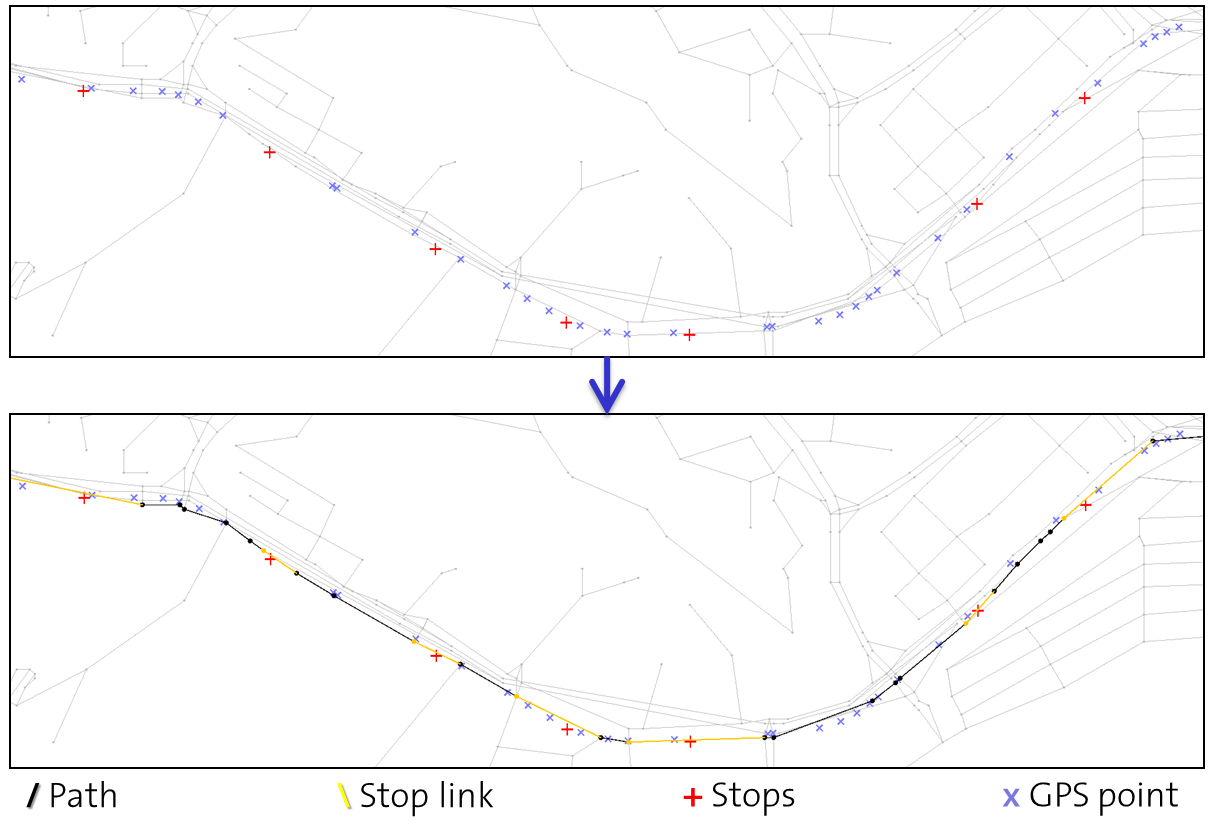
\includegraphics[width=1.0\textwidth]{extending/figures/semiAuto/Problem.png}}
{}

% .....................................................
\paragraph{Input Information}

The \gls{gtfs} is a recent but already widely used format for specifying public transport systems and was created by Google for feeding its geographic information applications. As of April~2011, the Singapore public transport system features 4\,584\,bus stops serviced by 355\,bus lines, all recorded on \gls{gtfs}. Each line has several routes, i.e. different outward and return routes due to one-way streets; as well as different coverage of serviced bus stops over weekdays and weekends. \gls{gtfs} records the name and location of each bus stop. For bus lines, it records constituent bus routes as a sequence of stops, along with its shape (a sequence of \gls{gps} points) as additional information. 

The \gls{gtfs} data needs to be mapped to a high resolution network; in the case of Singapore this is a navigation network developed by \gls{navteq}. The network is a directed graph where streets and intersections are represented as links and nodes. The links between nodes record attributes such as street name, number of lanes, length, flow, free speed, and capacity. Nodes are simply recorded as two-dimensional point coordinates. This network has a total of 79\,835\,links and 43\,118\,nodes.

% .....................................................
\paragraph{Special Restrictions}

There are some intrinsic characteristics of the public transport system that should be considered as hard restrictions to this problem. Firstly, when a certain stop is assigned to a link in the network, this link should belong to all paths related to routes to which this stop belongs. In other words: once established, stop-link relationships are fixed for resolving the missing routes. If the \gls{GPS} points from a route that includes a particular stop suggests it should rather be associated with a different nearby link, then all other routes involving that stop must be resolved again. Hence, the order in which the routes are resolved is important; it is preferable to resolve those routes first where we trust the quality of supporting information (\eg \gls{GPS} trails) best.

Secondly, while many lines are serviced in two directions, with most bus stops having a corresponding stop in the opposite direction (stop located on the other side of the street), this characteristic cannot be used to our advantage. This is because the links defined by each return route are different, the locations of stops are not necessarily exactly opposite to those in the opposite direction, and return routes  don't always use the same street.

However, some routes of the same line have an inclusion relationship: In peak hours, parts of bus routes facing high demand are serviced by additional bus services running on only partial routes to fulfil the demand. In these cases, if a full route is resolved, the solutions of its partial routes are included in its solution.

% ---------------------------------------------------------------------------
\subsubsection{Solution Approach}
It is not possible to automatically map-match the given \gls{gps} po with the network, as standard methods usually require at least 10\,points for each link \citep[][]{SchuesslerAxhausen_TechRep_IVT_2009}. In the Singapore \gls{gtfs}, the distance between consecutive points averages about 65\,meters, and the average link length is about 91\,meters, therefore we have fewer than 2\,points per link on average. Furthermore, the fact that not all the routes have \gls{gps} points inhibits using a full automatic solution; in the Singapore \gls{gtfs} there are 38\,bus routes without \gls{gps} points.

Consequently, the strategy for resolving each route consists of a semi-automatic procedure. Figure~\ref{fig:Process} illustrates the process. First, a simple map-matching algorithm is applied if the route is not part of a bigger route already solved (inclusion relationship described above). In this case, only a partition of a previous solution is needed for obtaining a first solution. Then, an automatic verification described below is performed. If the verification ends with a positive outcome, one can decide to finish the route and save the solution or to continue editing. If one decides, or is forced, to modify the solution there are two ways: changing parameters and running the automatic algorithm again, or editing the solution interactively with a graphical interface editing tool. In both cases the automatic verification must be executed again. If previously saved stop-link relationships are modified, prior routing solutions which contain one of the involved stops are erased.
%
\createfigure
{Semi-automatic process for one route}
{Semi-automatic process for one route}
{\label{fig:Process}}
{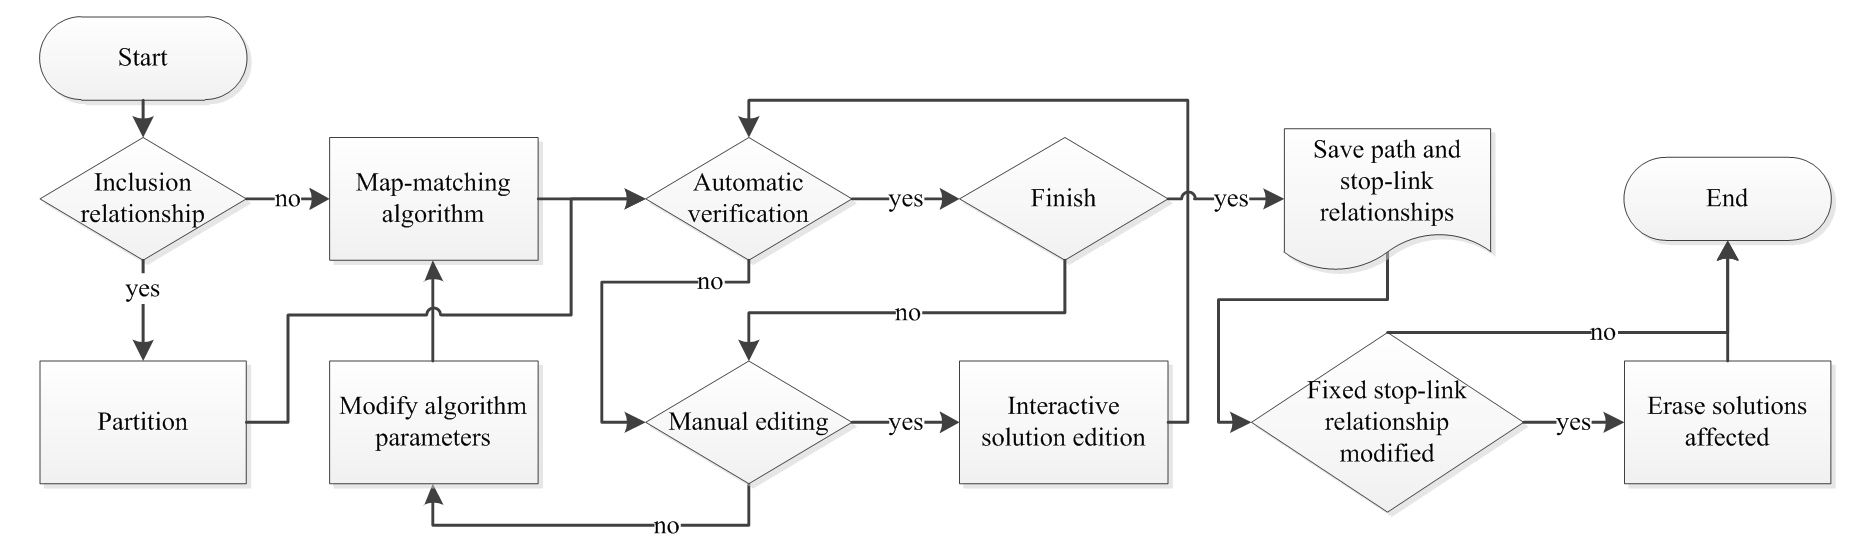
\includegraphics[width=1.0\textwidth]{extending/figures/semiAuto/Process.png}}
{}

As long as more solutions are obtained, it becomes easier and faster to solve further routes, similar to a  machine learning process. This happens for two reasons, firstly because of the inclusion relationships that omit the algorithm, and secondly because the increasing number of fixed stop-link relationships relaxes the algorithm. The functioning of the algorithm will be explained in the following section.

% ---------------------------------------------------------------------------
\subsubsection{Map-Matching Automatic Algorithm}
The objective of this algorithm is to generate a solution (path or sequence of connected links of the network, and a set of stop-link relationships) for one route, knowing its profile, a sequence of \gls{gps} points, and a set of stop-link relationships. The algorithm is designed to deal with:
%
\begin{itemize}\styleItemize
\item	Low resolution of \gls{gps} points;
\item	Sporadic low network spatial resolution;
\item	Long distances between two stops in the case of express routes;
\item	The fact that the nearest link to a stop point is not always the correct one.
\end{itemize}

The route map-matching process is illustrated in Figure~\ref{fig:Algorithm}. Except for the first stop, the algorithm solves for each stop in the route profile, a portion of the links sequence (from the previous to the current one) and, if this stop has no fixed link, a set of link candidates are pooled from which one link is selected.
%
\createfigure
{Map-matching algorithm}
{Map-matching algorithm}
{\label{fig:Algorithm}}
{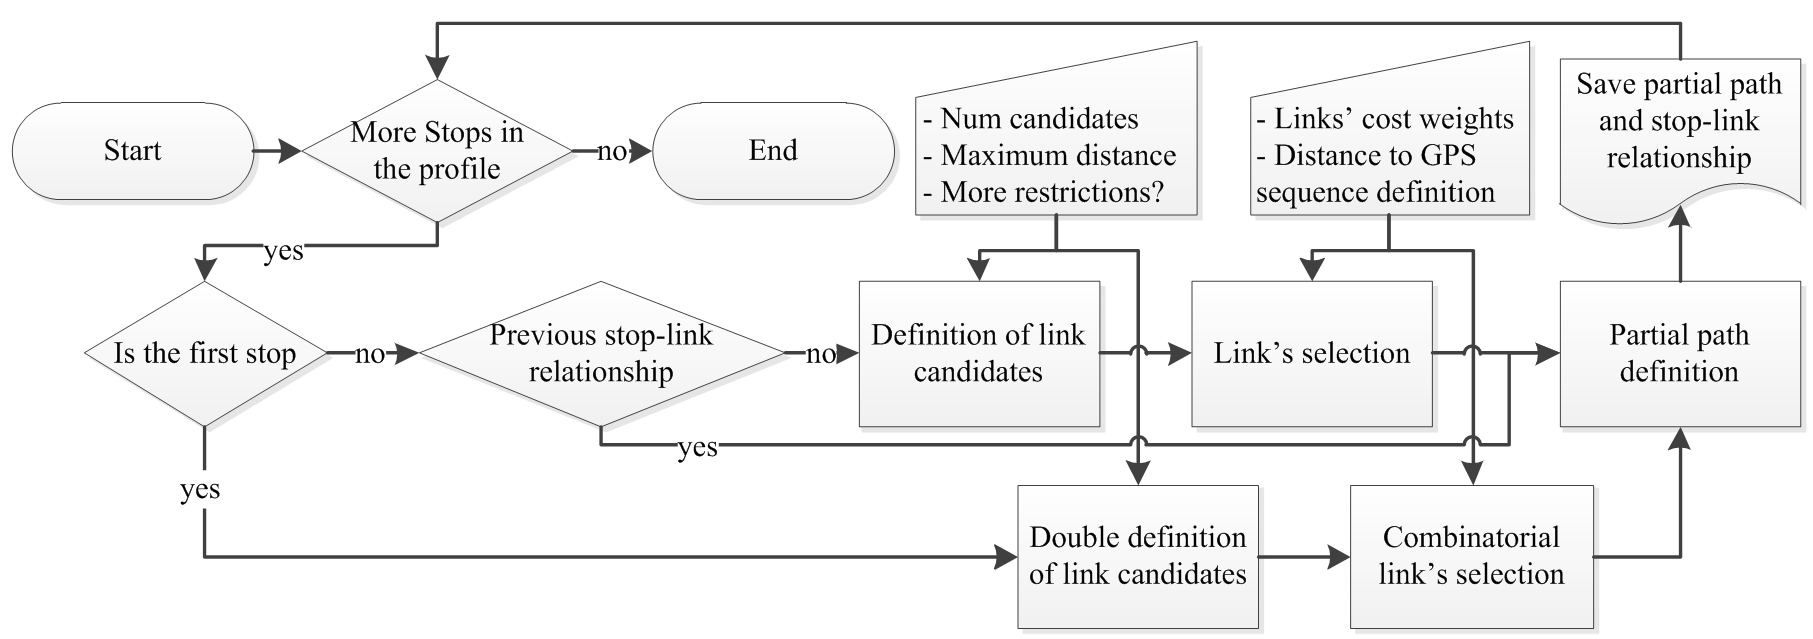
\includegraphics[width=1.0\textwidth]{extending/figures/semiAuto/Algorithm.png}}
{}

Definition of link candidates is performed as follows: the $NL$ closest links to the stop point, within a distance $D_{max}$, define a set of candidates. Each set's element could be subjected to more restrictions: the nearest point between the stop point and the infinite line defined by the link, must be inside its line segment, and the angle between the link direction and the nearest GPS points sequence direction must be lower than $\alpha_{max}$.

The link's selection is performed as follows: from the previous stop link to each defined candidate, an A star search algorithm is applied for finding the shortest path. For running this algorithm, each link cost depends on the link's travel time and the distance from the link to the \gls{gps} points. A product with flexible exponents was proposed a first model:
%
\begin{equation}
\label{eq:LinkCost}
	C_{link} = \exp{\frac{L_{link}}{S_{link}}}{w_{1}}\exp{D_{GPS}}{w_{2}}
\end{equation}
%
where $L_{link}$ is its length, $S_{link}$ is its free speed, $D_{GPS}$ is its distance to the \gls{gps} points sequence, and $w_{1}$ and $w_{2}$ are positive weights with a standard value of 1, but modifiable by the user according to the existence or quality of the \gls{gps} points sequence. The definition of $D_{GPS}$ can be modified; in the simplest approach it is the minimum distance between the link and all the \gls{gps} points (point-segment distance). From all the calculated paths the shortest one is selected and added to the general solution of the route. The corresponding link candidate is also related to the stop. 

If the current stop had a stop-link relationship, only the shortest path to this stop defines the solution. Thus, the process continues with the next stop in the route profile. If the first stop of the profile has no fixed link, a similar algorithm between the first and the second stop is performed. The definition of candidates procedure is applied to the first and the second stops. Then, the candidates' selection procedure consists of obtaining the shortest path of all the combinations between the two sets of candidates, and selecting the shortest one. This path defines links for both stops.

% ---------------------------------------------------------------------------
\subsubsection{Automatic Verification}
In this step, the correctness of the routing solution is automatically checked by performing the following, ordered verification:
%
\begin{enumerate}\styleEnumerate
\item Is the path joined?
\item Is the path without U turns?
\item Is the path without repeated links?
\item Does every stop of the route have a stop-link relationship?
\item Is every link related to a stop inside the path?
\item Is the order of the related links in the path the same as the order of the corresponding stops in the route profile?
\item Is the nearest point between the stop point and the infinite line defined by the link inside its line segment in every stop-link relationship?
\item Are the first and last links of the path related to the first and last  stops of the route profile?
\end{enumerate}

Verifications (2), (3) and (7) are not mandatory and can be deactivated through the user interface. User interaction is necessary to (i) cover possible errors, and (ii) include actual route characteristics: some bus routes indeed present U turns, some repeat exactly the same street in the same direction during their travel, and the geometric restriction presented in (7) is not always valid in big stop facilities like bus interchanges.

% ---------------------------------------------------------------------------
\subsubsection{Manual Editing Functionalities and Implemented Software}
The objective of the edit functions is to allow the user to modify the automatically generated routing solution. Even if the automatic algorithm generates a correct solution based on the input data, problems such as recent changes in routes, differences in the release date between \gls{gps} points and network data, erroneous \gls{gps} points, or lack of network elements require manual changes. Although one also could modify and correct the input data or the generated solution with direct data modifications, two-dimensional visualization and keyboard-mouse user interaction are two quality attributes which help to reduce time and effort. Developed functional requirements and quality attributes are described as follows:
%
\begin{enumerate}\styleEnumerate
\item Visualization: A navigation network is displayed, including all relevant information for working with a single route. This includes the route's profile, the given sequence of \gls{gps} points, and its current solution (path and stop-link relationships). Selected elements are drawn in a different color. Everything is displayed in a two-dimensional and interactive way, including the location of the cursor in working coordinates, panning, zoom and view-all options.
%
\item Selection: Different options for selecting elements of the solution, or elements from the network, are provided. It is possible to select the nearest link from the solution or from the network, the nearest node from the network, or the nearest stop from the solution, to a point indicated by the user. When a stop that already has a stop-link relationship is displayed, its corresponding link is highlighted as well. If a link of the solution path is selected and it does not have a subsequent link connected, a new one from the network is selected with one click; the selected link is the one with the most similar angle to the line defined by the end node of the initial link and a point indicated by the user.
%
\item Path modification: The first link of the sequence can be added by selecting any link of the network. If a link of the solution path does not have a subsequent link connected, it is possible to add one according to the selection function described in (2). If there are two sequential links in the solution that are not connected (a gap), a sub-sequence that connects the mentioned links is added, using the shortest path algorithm, with the current parameters. Furthermore, selecting one link of the solution path, it is possible to delete it, or to delete all the links before or after it. Finally, stop-link relationships can be modified by selecting either elements. If the modified relationship was fixed, the user is prevented from modifying the relationship because the tool will erase the solutions of the routes to which the selected stop belongs.
%
\item Network modification: New nodes to the road network can be added. In addition, with any node selected, it is possible to add a new link selecting the end node.
\end{enumerate}

These functions were implemented in a software package developed from scratch in \gls{java} and using the Java2D library for graphics. It reproduces the described solution approach, looking for non-solved routes, and running the map-matching algorithm and the automatic verification for each one. Figure~\ref{fig:Application} shows the user interface and a demo video can be accessed at \url{http://www.vimeo.com/27137889}.

\createfigure
{User interface of the application to edit automatic solutions}
{User interface of the application to edit automatic solutions}
{\label{fig:Application}}
{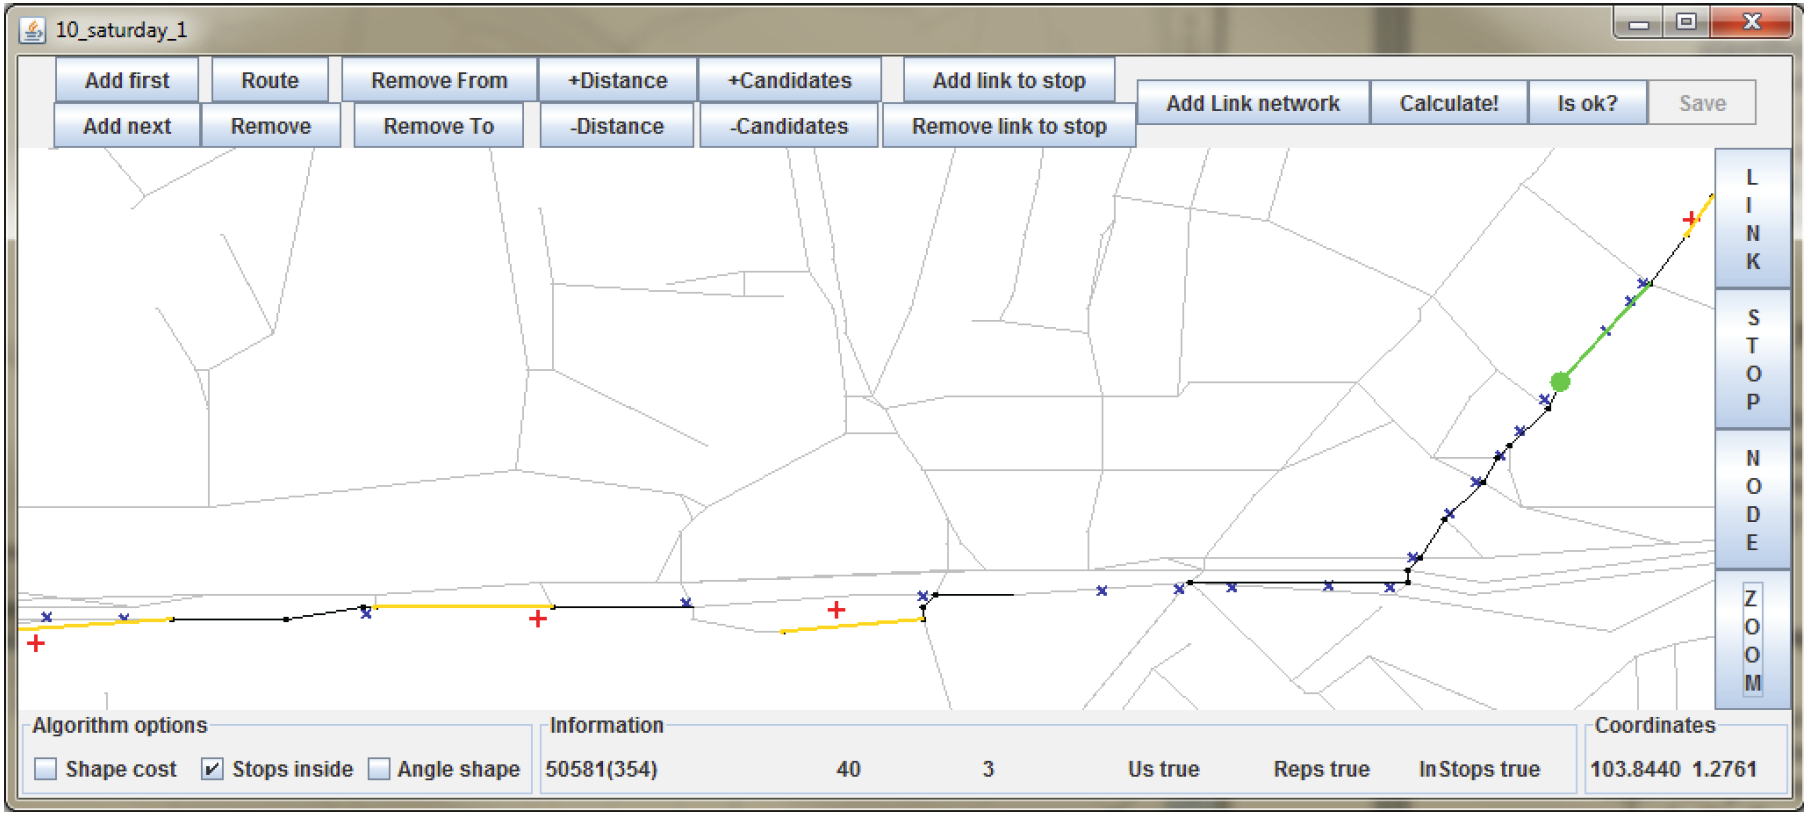
\includegraphics[width=1.0\textwidth]{extending/figures/semiAuto/Application.png}}
{}

% ---------------------------------------------------------------------------
\subsubsection{Conclusion and Outlook}
The semi-automatic procedure designed for map-matching bus lines with a high resolution navigation in Singapore was successful, allowing to solve all bus routes and stops in only ten days. This is taking into account the quality of the input information offered, highlighting the low spatial and temporal resolution of the \gls{gps} points given for each route. Analysis of the process reveals that reducing the manual modification time is the best way to improve the procedure. It can be done by modifying the automatic algorithm for obtaining more accurate results for the initial routes to be solved, or in other words, for routes not affected by the learning process.

As \gls{gtfs} is becoming so popular for defining public transport systems and the code in which this process is implemented, is open source, it can be used for matching routes with high resolution networks of any \gls{gtfs}-specified place. The tools are available as a \gls{matsim} \gls{contribution} (\lstinline|GTFS2TransitSchedule|). For generating \gls{matsim} simulation scenarios the presented procedures have been used by a research team in the province of Gauteng, South Africa, the Toronto scenario and a different public transport simulation model developed by SMART-MIT in Singapore.

% ============================================================================================
\subsection{New Dynamic Events-Based Public Transport Router}
In public transport route choice, the decisions and actions of a particular user depend not only on their own preferences (value of time, crowd avoidance, willingness to pay). They also depend on the decisions and actions of many other public transport users, operators and authorities. Even the decisions of private transport users are also involved, as everybody shares the same infrastructure.

The current implementation of \gls{matsim} implements a \gls{sbptr} as mentioned above. It means, when an agent needs a route for a given start time, origin and destination, the \gls{sbptr} finds the shortest path in a schedule-based network assuming public transport vehicles are always on time and always have space. Within the mobility simulation a given vehicle can arrive early or late and/or it can be full, thus not allowing additional passengers to board. Hence, when a bad experience happens, the agent obtains a bad score and it is possible this plan will get replace with a more favorable one during the iterative learning process. The problem is that if the agent tries to find a new route for the same start time, origin and destination, the shortest path in the public transport scheduled network is going to be the same, and agents can not improve their experiences by changing the route.

To address this shortcoming, a new \gls{ebptr} is proposed \citep[][]{OrdonezErath_TechRep_FCL_2013}, modeled, implemented and tested. It takes the given schedule as a base for the first iteration, but updated information on travel times, occupancy of the public transport vehicles, and waiting times is propagated between subsequent iterations. Thus, when executions of the same day are performed, new routes can be generated for the same start time, origin and destination, because the system is remembering delayed bus services (longer travel times), or train services where the vehicle arrives full (longer waiting times). However, the network within agents are routed needs a new topology to account for such variables. This approach allows then to account for emergent phenomena: in situations where overcrowded vehicles prohibit boarding, it makes sense for some agents to travel for a few stops in the outbound direction to transfer to a vehicle with sufficient capacity heading inbound to be able to board. Although more memory is needed, similar or even better computation times are achieved when shortest path calculations are performed due to the simpler network topology. Furthermore, to achieve user equilibrium requires a significantly fewer number of iterations.

% ---------------------------------------------------------------------------
\subsubsection{Events-Based Public Transport Router} 
\label{sec:RouterStructure}
A new \gls{ebptr} was developed for \gls{matsim} with the objective of modeling more realistic public transport route choice, where agents learn over time that the transit vehicles are not always on time, do not always have sufficient space to allow for boarding a vehicle and trips with more comfort can be preferred.

% .....................................................
\paragraph{Network Topology}

Figure~\ref{fig:Networks}(b) shows the structure of the proposed public transport network compared with the original structure (Figure~\ref{fig:Networks}(a)). Inspired by the network designed by \citet{SpiessFlorian_TransResB_1989} this implementation has two types of nodes. The first type represents a stop facility (green-black squares) as point in space while the second type (yellow-red dots)represents stop-route relation which can be seen as a physical or virtual platform for each line which passes a particular stop facility. For example different platforms in a metro system need to be modeled as different stop facilities because different services arrive at each platform and walking paths are needed to change from one platform to another. For bus stop facilities, they represent virtual platforms as in reality buses of different lines serving the same bus stop will normally use the same physical infrastructure \eg a bus bay. To connect those nodes, there are four types of links. The in-vehicle links join two consecutive stop-route nodes in the direction of the correspondent route. The boarding links connect a stop node with each corresponding stop-route node. The alighting links are the opposite, so they connect the stop-route nodes with their corresponding stop node. Finally walking links connect a stop node with all the other stop nodes located within a walkable distance.

\createfigure
{Comparison of the network topologies}
{Comparison of the network topologies of the schedule-based transit router (a) and the new events-based transit router (b).}
{\label{fig:Networks}}
{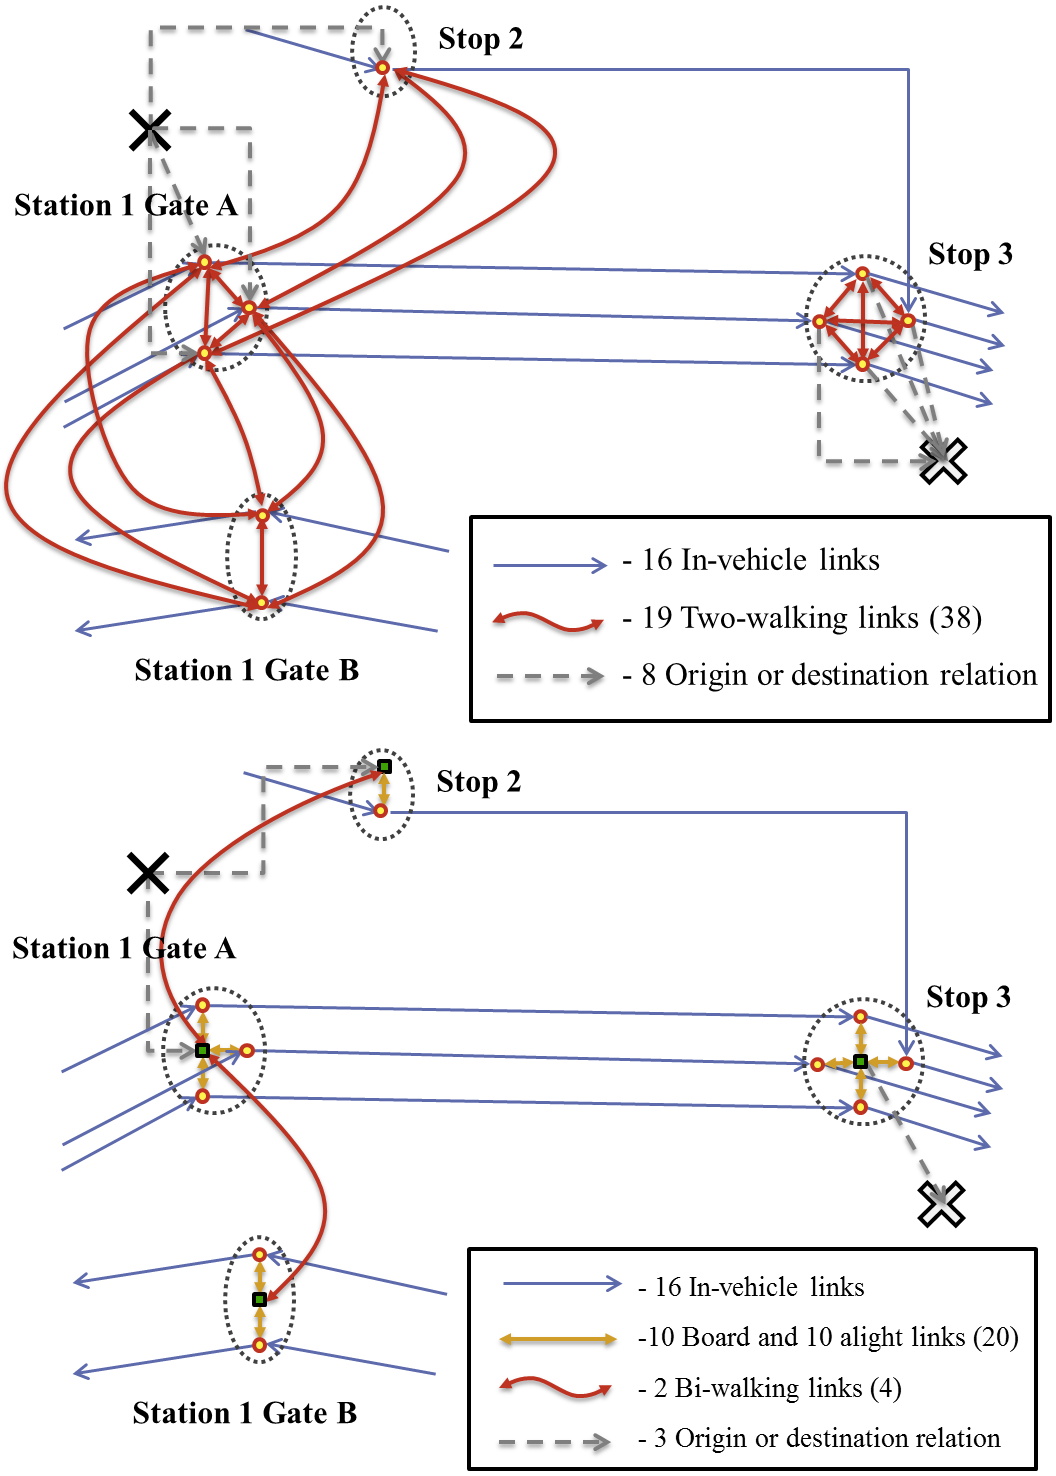
\includegraphics[width=1.0\textwidth]{extending/figures/ebr/Networks.png}}
{}

% .....................................................
\paragraph{Link Costs}

Each link in this network has a related time-dependent disutility function. Different costs are saved for different times in the day for a given time bin (currently 15\,minutes). In-vehicle link disutilities depend on the vehicle travel time, the travel distance, the level of occupancy and a fare rate if this system is distance-based. Boarding links disutilities depend on waiting times, a transfer cost, and a fixed fare if this system is entry-based; thus it is possible to relate specific stop-route waiting times to these links. As the first waiting link is not a transfer, this cost has to be subtracted from the whole path cost, but this detail does not affect the shortest path calculation. Alighting links don't have any cost associated, but it is possible to relate a fare to them. Finally, walking links depend on the walking travel time and distance. Equation~(\ref{eq:CostFunction}) shows linear versions of these functions used in this model assuming a distance-based fare system.
%
\begin{equation}\label{eq:CostFunction}
	\begin{array}{l}
		C_{iv}(t) = (\beta_{iv}*t_{iv}(t))(1+g(p_{oc}(t))) + \beta_{vd}*l_{iv} + f_{iv}*l_{iv}\\
		C_{bo}(t) = \beta_{wt}*t_{wt}(t)) + c_{tr}\\
		C_{al}(t) = 0\\
		C_{wk}(t) = \beta_{wk}*t_{wk} + \beta_{wd}*l_{wk}\\
		C_{path}(t) = \sum{C_{iv}(t')} + \sum{C_{bo}(t')} + \sum{C_{al}(t')} + \sum{C_{tr}(t')} - c_{tr}
	\end{array}
\end{equation}

$C_{path}$: Total cost of the path.

$C_{iv}$: Cost of one in-vehicle link.

$C_{bo}$: Cost of one boarding link.

$C_{al}$: Cost of one alighting link.

$C_{wk}$: Cost of one walking link.

$\beta_{iv}$: Personalized cost per unit of time traveling in a vehicle.

$\beta_{vd}$: Personalized cost per unit of distance traveling in a vehicle.

$\beta_{wt}$: Personalized cost per unit of time waiting in a stop.

$\beta_{wk}$: Personalized cost per unit of time walking.

$\beta_{wd}$: Personalized cost per unit of distance walking.

$c_{tr}$: Personalized cost for make a transfer

$f_{iv}$: Vehicle dependent fare rate by distance traveled

$t_{iv}(t)$: In-vehicle travel time (from Stop-stop travel times structure).

$t_{wt}(t)$: Waiting time (from Stop-route waiting times structure).

$t_{wk}$: Walking time.

$l_{iv}$: In-vehicle distance.

$l_{wk}$: Walking distance.

$p_{oc}(t)$: Occupancy level in the in-vehicle link (from Route-stop occupancy structure).

$g(p)$: Simplified function of how occupancy level increases the cost (Equation~(\ref{eq:Occupancy}))

\begin{equation}\label{eq:Occupancy}
	g(p)=\left\{\begin{array}{l}
	0\hspace{25 mm}if\hspace{5 mm}p \leq p_{sit} \\
	r_{sta}*p + b_{sta}\hspace{5 mm} if\hspace{5 mm}p_{sit}<p<1\\
	b_{full}\hspace{20 mm} if\hspace{5 mm}p=1
	\end{array}\right.
\end{equation}

$p_{sit}$: Occupancy level when no more seats are available.

$r_{sta}, b_{sta}$: Parameters of percentage increase in discomfort from standing in the vehicle.

$b_{full}$: Maximum percentage increase when the vehicle is full.

% .....................................................
\paragraph{Shortest Path Algorithm}

To find a public transport route between an origin and a destination for a given time in the day the applied method is the same as currently implemented in \gls{matsim}: first, the algorithm looks for the stop-nodes within a walkable distance from the origin and from the destination. An initial cost is associated with each of these stop-nodes according to access and egress walking times. Then, starting from all the origin-stop-nodes with a given access cost, a multi-node time dependent Dijkstra algorithm finds the shortest path, to the destination-stop-nodes with related egress costs. Thus, the path determines the best \gls{od} combination as well. The algorithm is time-dependent because it takes into account that time is advancing while it proceeds through the path; thus, different costs are obtained from the links while time is advancing. The total disutility of this path is compared with the cost of a full walking trip. If the cost is less, the path is converted to a sequence of stages: in-vehicle stages for each in-vehicle link in the path and walking stages for each walking link. Boarding and alighting links are ignored for this conversion.

% .....................................................
\paragraph{Structures to Save Travel Times, Waiting Times and Vehicle Occupancy} 
\label{subsec:Structures}

As mentioned earlier, the \gls{mobsim} of \gls{matsim} generates atomic units of information called \glspl{event}, which describe state changes for each person, \eg boarding and each vehicle, \eg entering and leaving a link during the course of the simulation. The objective of this work is to save information of the public transport experience in one simulation to find better public transport routes for the agents in the next iteration. This feedback mechanism is already implemented in \gls{matsim} for private transport. The car router uses time-dependent travel times of each link saved in a previous iteration to calculate better routes in the road network, by changing the costs of the links. To allow the \gls{ebptr} to learn from the previous iteration, information about a) stop-stop travel times, b) stop-route waiting times and c) route-stop-stop vehicle occupancy, is required.

\begin{itemize}\styleItemize
\item Stop-stop travel times: In order to account for delays of public transport vehicles, the travel time between consecutive stops must be saved. Two stops are consecutive if they are consecutive at least for one public transport route. A first option is to use the mentioned travel times structure that saves time-dependent travel times for each link in the road network. As the road links a vehicle has to follow between two consecutive stops are known these travel times can be summed. The problem is that this structure takes into account all the vehicles in the network, and particularly in the links where public transport stops are located, travel times of cars and buses are very different. Consequently a special structure was implemented to save these stop-stop travel times. The structure averages all the public transport vehicle times from one stop to a consecutive one during a certain time bin in the day. More specifically, each value comprises the time since the vehicle arrived at a certain stop until the vehicle arrives at the consecutive stop, denoted in the simulation by consecutive \lstinline|VehicleArrivesAtFacility| events. This means that the first stop dwelling time and all the queue times (if the vehicle has to queue before the bay or platform is available) are included. In other words, when an agent is routing the first in-vehicle link of each trip, the full dwell time will be included. Hence this agent is assuming it is the first passenger entering to the vehicle. For all the other in-vehicle links the in-vehicle waiting is included. These stop-stop times are the main component of the in-vehicle link disutilities.
%
\item Stop-route waiting times: Waiting times are a fundamental aspect in public transport route choice. Waiting times can be long due to vehicle delays (\ie due to the stop location), or when public transport vehicles of one or several consecutive services are full (\ie due to the route demand and stop position within the route). For that reason waiting times are saved for each stop-route relation. Similarly, the structure averages all the agent waiting times in a certain stop for a certain route during a certain time bin in the day. More specifically each value comprises the time since the agent arrives to the public transport stop until it enters the vehicle, denoted in the simulation by consecutive \lstinline|AgentArrivesToFacility| and \lstinline|PersonEnterVehicle| \glspl{event}. These waiting times are the principal component of the boarding link disutilities. If no observations are found for a certain stop-route-time the model saves a half of the corresponding headway, specified by the transit schedule.
%
\item Route-stop occupancy: To account for the occupancy level allows to model routing decisions where people take in terms of travel times longer routes in order to feel more comfortable in emptier vehicles, \eg valuing a higher chance to travel seating. Occupancy depends on the demand of a certain route and the position of the stop within the route. The occupancy is assumed constant between two consecutive stops. When a vehicle departs from a certain stop (denoted in the simulation as \lstinline|VehicleDepartsFromFacility| event) this structure averages the occupancy level with the other vehicles of the same route that departed from the same stop during the same time bin. As there are few vehicles for each time bin it is very likely not to find observations for a certain time bin. In this case the structure returns the value of the next time bin where at least one observation is found of the corresponding stop and route.
\end{itemize}

% ---------------------------------------------------------------------------
\subsubsection{Functional Results}
\paragraph{Relaxation Process}

The number of iterations needed by \gls{matsim}'s co-evolutionary algorithm to reach a stable state is a critical variable; efforts have been performed to reduce it \citep{MeisterEtAl_STRC_2006, FourieEtAl_TRB_2013}.

The \gls{ebptr} effectively reduces the number of iterations public transport users need to reach equilibrium. Using a 25\,\% of the Singapore scenario, Figure~\ref{fig:Relaxation} shows the evolution of average scores of the plans of 355\,207\,agents trough 100\,iterations. These 100\,iterations were executed four different times to use both routers for two different replanning strategies. Agents are saving five plans in memory. At iteration~0, both \gls{ebptr} and \gls{sbptr} start with routes as described in the schedule; however, the \gls{ebptr} returns routes which perform better in this first simulation. This occurs because for each pair consecutive stops the \gls{ebptr} uses the average between all the scheduled times of the routes which contain this pair as the first estimate. On the other hand, the \gls{sbptr} uses the specific scheduled time of the corresponding route. According to the results the average stop-stop time seems to be a more reliable estimate for this first iteration.
\createfigure
{Comparison of score evolution}
{Comparison of score evolution: a) 30\,\% re-route, b) 20\,\% re-route and 10\,\% time allocation}
{\label{fig:Relaxation}}
{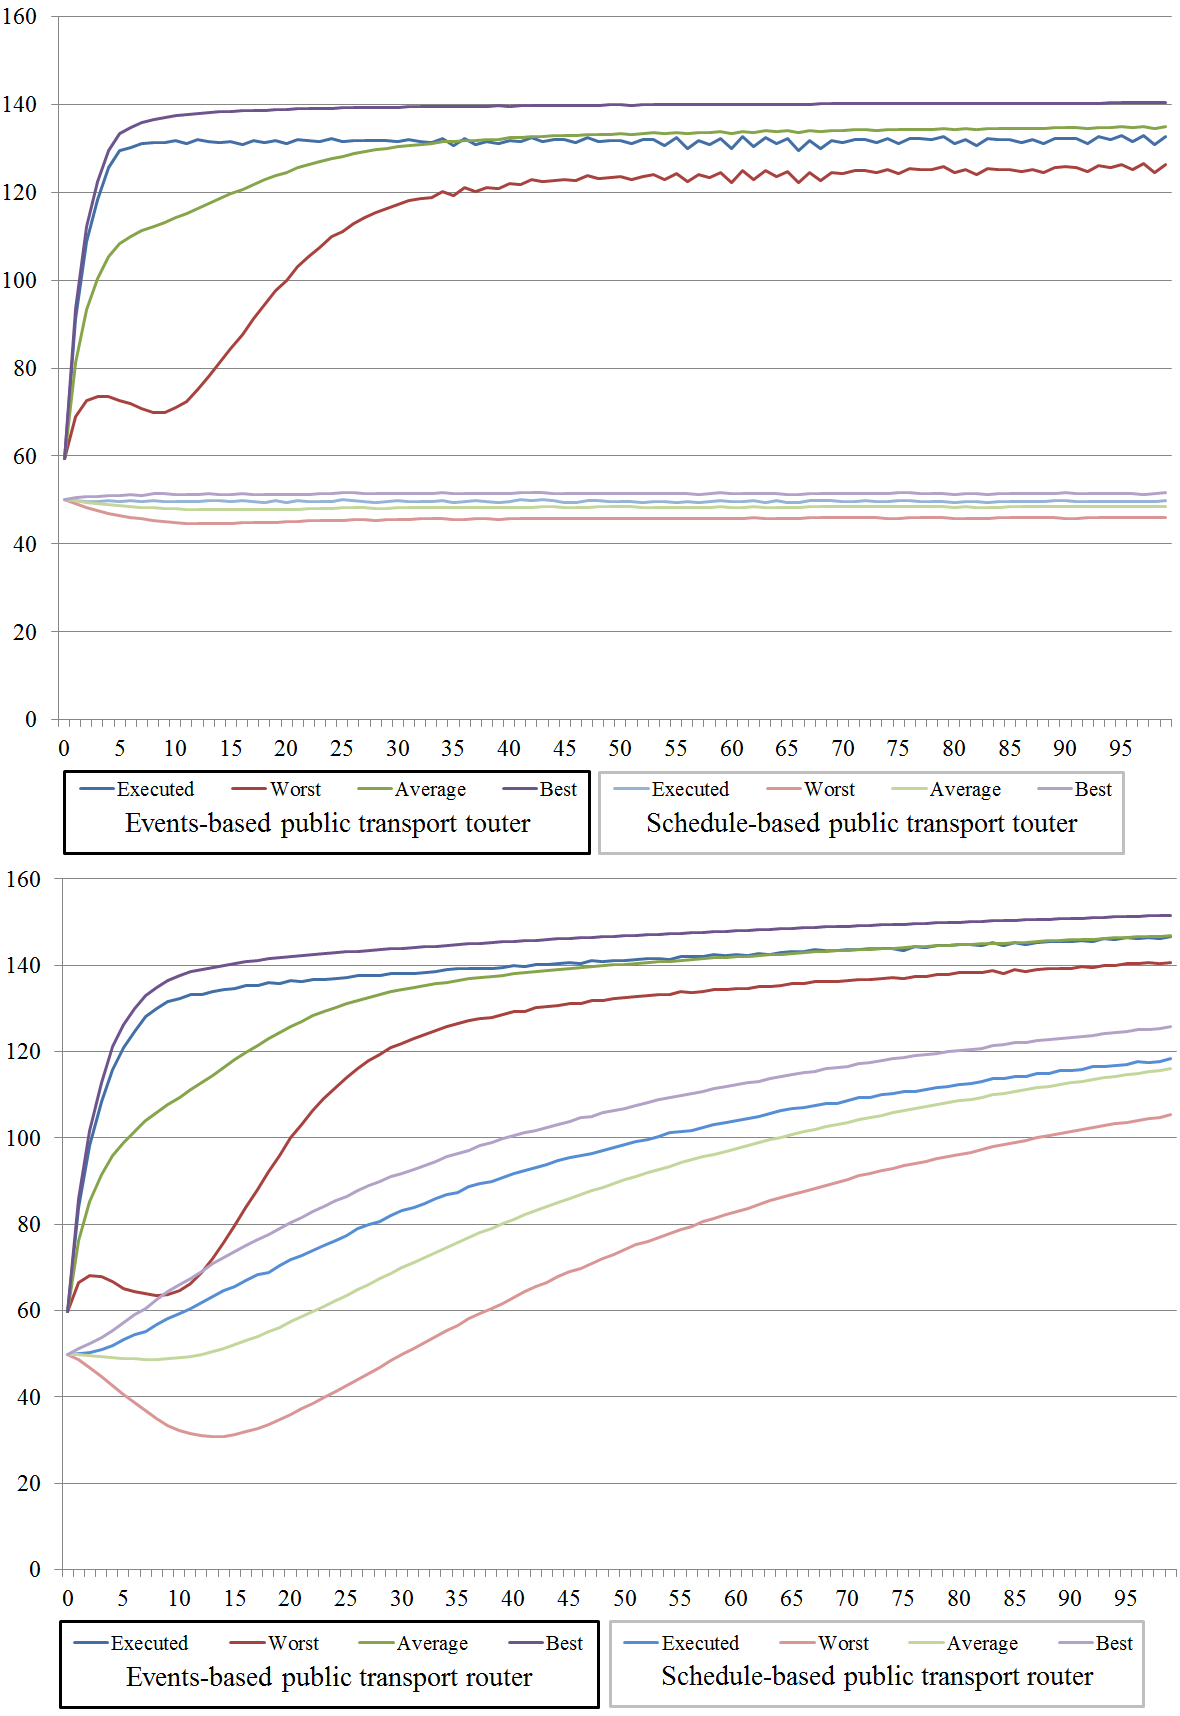
\includegraphics[width=1.0\textwidth]{extending/figures/ebr/Relaxation.png}}
{}

Now, for the rest of the iterations, the Figure~\ref{fig:Relaxation} shows how the scores evolve. The first replanning strategy stipulates that 30\,\% of the agents are re-routed at each iteration. This evolution is shown in the first graph of the figure. Using \gls{sbptr}, agents receive the same route over and over again as the start time origin and destination do not change between iterations. Small variations in scores occur because of the stochastic nature of the simulation explained above. Although scores start in the same range, using \gls{ebptr} caused that better performing routes are found within a very small number of iterations.

For a more realistic comparison a second replanning strategy is tested, where just 20\,\% of the agents are re-routed and the activity start times are modified randomly within a half an hour for 10\,\% of them. The second graph of the figure shows how both routers manage to improve agents' plan scores. But with the \gls{ebptr} the number of iterations needed to achieve the average executed score achieved after 100\,iterations for the \gls{sbptr} (120) was just 5. The marginal score (as a measurement of relaxation advance) after 200\,iterations with the \gls{sbptr} (0.1\,utility point per iteration) is achieved after 77\,iterations with the \gls{ebptr}. This means an improvement by a factor of 2.6.

% .....................................................
\paragraph{Modeling Advantages}

As the disutility function of the links in the proposed network account for aspects like waiting times or occupancy levels, and as \gls{matsim} allows to model heterogeneity among agents, the router results in a very powerful tool to model emergent behavior in public transport route choice as observed in the reality. In Singapore, as many other crowded cities in the world, some people decide to travel backwards for a few stops and transfer to a train in the opposite direction to find a seat or space in a public transport vehicle \cite{ChakirovErath_HKSTS_2011}. With the \gls{sbptr} such type of least cost path can not be found, but with the new proposal this is possible. Although proportions do not match with actual observations as the Singapore scenario lacks of appropriate and calibrated utility parameters for traveling and waiting time under crowed conditions, Figure~\ref{fig:Backwards} shows totals of people traveling backwards from different stops in the island after 100\,iterations (see Figure~\ref{fig:Relaxation} (a)).

\createfigure
{Number of agents traveling backwards at each \protect\gls{mrt} station of the Singaporean rail system}
{Number of agents traveling backwards at each \protect\gls{mrt} station of the Singaporean rail system}
{\label{fig:Backwards}}
{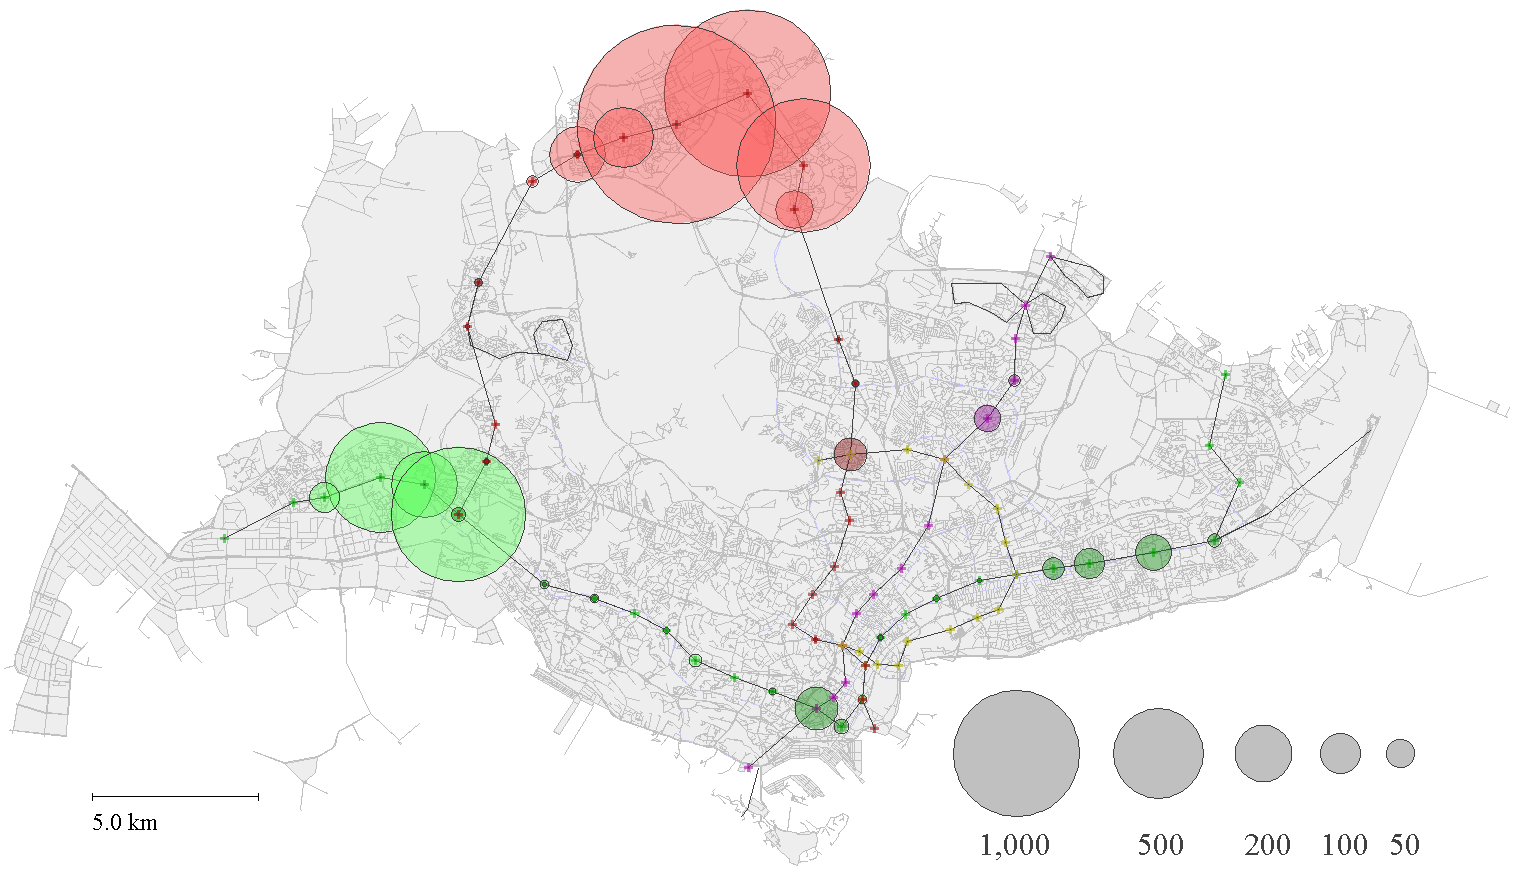
\includegraphics[width=1.0\textwidth]{extending/figures/ebr/Backwards.png}}
{}

\subsubsection{Comparing Quality Attributes With the Current Implementation}

% .....................................................
\paragraph{Computation Time}

The tests described next were executed using 12\,computational nodes, accessing 70\,\gls{gb} of shared memory, and using the Singapore scenario described in Chapter~\ref{ch:singapore}. Before the first iteration, if plans are not routed, \gls{matsim} prepares every agent with an initial route. As it was mentioned before, the stop-stop travel times and stop-route waiting times are initially taken from the schedule. Because of its simpler network structure the \gls{ebptr} takes 01:17:35 to initially route the 355\,207 users compared with 01:28:55 needed by the \gls{sbptr} which equals to a gain of about 12.7\,\% for this scenario. When running \gls{matsim} iterations with the \gls{ebptr}, computation times principally change in two processes: mobility simulation (mobsim) and replanning. Figure \ref{fig:CompTimes} shows computation times measured for the first 20\,iterations of the process. Although the \gls{ebptr} needs more time in \gls{mobsim}, it continues to require considerably less time for re-routing during the replanning due to a simpler network topology. The longer mobsim time is due to the saving of information in the mentioned new structures during the course of the simulation. However, in average the \gls{ebptr} outperforms \gls{sbptr} per iteration by about 3\,minutes or 11\,\%. As mentioned above 2.6\,times more iterations are needed for the \gls{sbptr} to achieve a specific point in the relaxation process. For 77\,iterations with the \gls{ebptr}, the computation amounts 35:25:43, and for 200\,iterations with the \gls{sbptr} the computation amounts 99:10:51; that is an improvement by a factor of 2.8 in our experimental setting.

\createfigure
{Comparison of computation times for 20\,iterations}
{Comparison of computation times for 20\,iterations}
{\label{fig:CompTimes}}
{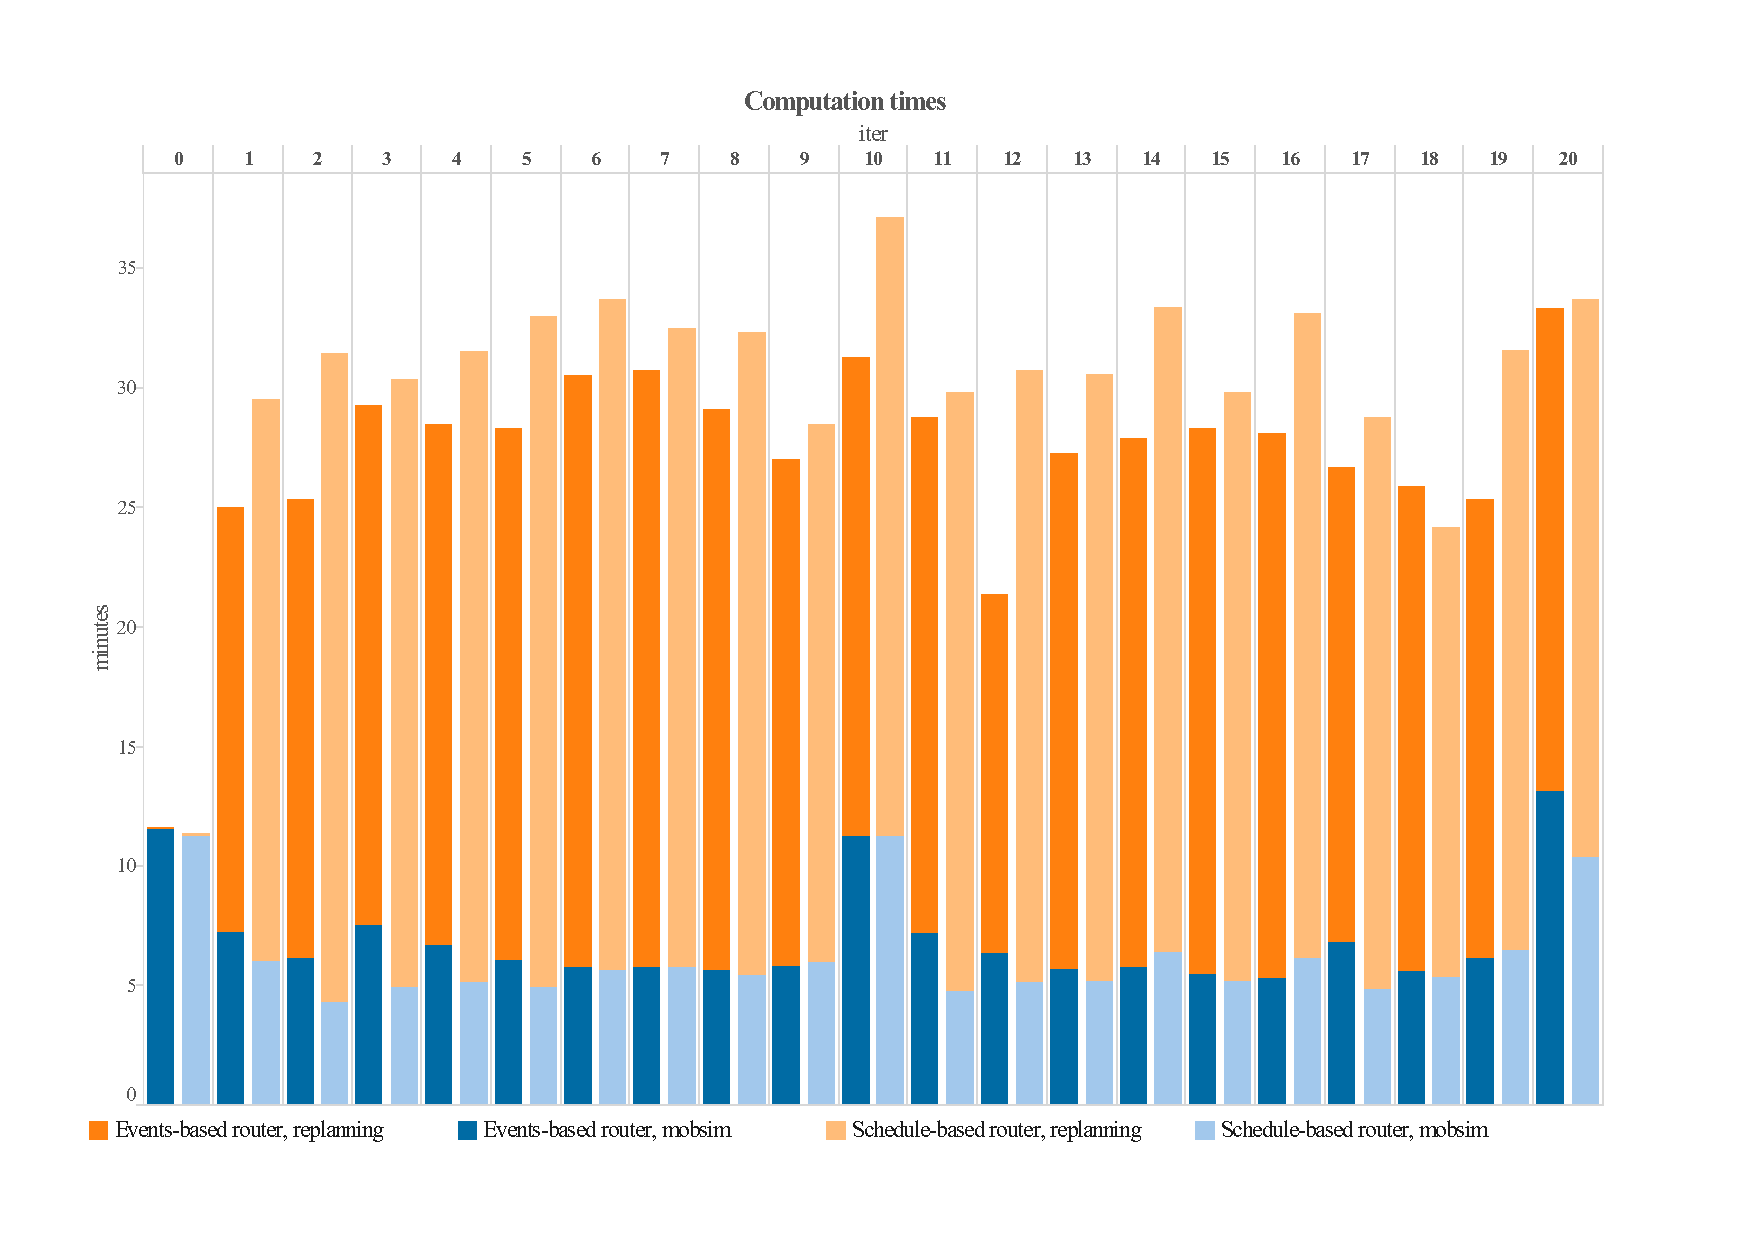
\includegraphics[width=1.0\textwidth]{extending/figures/ebr/ComputationTimes.pdf}}
{}

% .....................................................
\paragraph{Memory Consumption}

The \gls{ebptr} needs more memory than the \gls{sbptr} because the \gls{ebptr} manages more information. The necessary extra memory is allocated to the three structures described before. Given the conditions described for the Singapore scenario the extra memory is calculated as follows. One numeric value needs eight Bytes, and with a time bin of 15\,minutes, 120\,bins are needed for 30\,hours. The Stop-stop travel times structure saves two values (average and number of observations) per each time bin per each pair of consecutive stops. The number of pairs for the Singaporean public transport system is 6\,602. Thus, this structure approximately needs 12.7\,\gls{mb}. Similarly, The stop-route waiting time structure saves two values (average and number of observations) per each time bin per each pair of stop route combinations. The number of stop-route relations for the Singaporean public transport system is 27\,156. Thus, this structure needs approximately 52.1\,\gls{mb}. Finally, the vehicle occupancy structure saves the average and the number of observations for 26\,353\,route-stop relations for each of the 120\,time bins. Hence it requires approximately 50.7\,\gls{mb}. In total less than 120\,\gls{mb} are needed for the three structures.

On the other hand the size of the network where public transport routes are calculated is smaller for the \gls{ebptr}. Although, in the case of Singapore, it creates 31\,939\,nodes compared with 27\,156 of the \gls{sbptr} (4\,783 new stop-nodes) the number of links is dramatically smaller. The \gls{sbptr} creates 424\,070\,walking links and 26\,353\,travel links (450\,423 in total). The \gls{ebptr} creates the same 26\,353\,travel links, plus 27\,156\,boarding links, plus 27\,156\,alighting links and just 4\,390\,walking links (85\,055\,links in total); less than a fifth in total. As a node needs 48\,bytes and a link 128\,bytes approximately the \gls{sbptr} needs 46.8\,\gls{mb} more memory for links and just 229.6\,KB less for nodes. The \gls{ebptr} saves 46.5\,\gls{mb} for the network, concluding that in total the \gls{sbptr} needs 70\,\gls{mb} less memory. This quantity in neglectable compared with the total memory needed for the whole process (more than 40\,\gls{gb}).

% ---------------------------------------------------------------------------
\subsubsection{Conclusion and Future Work} 
\label{sec:ConclusionsAndOutlook}
In this work a new public transport router for \gls{matsim} was designed, implemented and tested. It allows to obtain more diverse routes in large scale scenarios taking into account many complexities of urban public transport systems. On the supply side, the system simulates congestion, occupancy levels of public transport vehicles, queues in public transport stops, bay sizes, and bus or train bunching. On the demand side, in addition to the commonly used factors such as in-vehicle time, number of transfers and walking time, the presented new router takes into account disutility of additional waiting time due to congestion or overcrowded vehicles, comfort level inside public transport vehicles and preference heterogeneity among agents for all mentioned factors.

The usability of the new approach was tested in a large scale scenario of Singapore. Using a simplified public transport only simulation, 100\,iterations of a 25\,\% scenario (355\,207 agents) with 30\,\% of the agents re-routing each iteration took just 45\,hours approximately, or about 27\,minutes per iteration, using 12\,cores and 70\,\gls{gb} of memory. The computation was improved compared to the standard \gls{matsim} in 11\,\% less. If just 20\,\% of the plans are re-routed and using 35\,cores accessing 85\,\gls{gb} of memory, the time per iteration is reduced to less than 13\,minutes, achieving 100\,iterations in less than one day. But in terms of computation time gains most importantly, we showed that the proposed events-based router is able to reach a steady in a much smaller number of iterations.

If the proposed router works better than the original one, is it worth to change it? Well, the current scheduled-based router of \gls{matsim} would still be relevant if the topology of its network is changed for the proposed one. It also should be applied to scenarios where the public transport system operates at a very reliable time table, with little situations of overcrowding. In that case routing calculations would be as fast as the events-based router (with the new network structure), and the mobility simulation would be faster as no information (in-vehicle time, wait time and occupancy) would be needed. In other words, it can be applied to models of cities where public transport users can plan their trips using just a time table.

In terms of the resulting network loading, the potentially biggest advantage of the proposed events-based router is its capacity to generate emergent behavior in congested public transport systems which is in line to actual observations. Future research should aim at estimating the various route choice behavior parameters corresponding to the provided functionalities of the proposed system and calibrate the simulation. Although the currently used values came from a stated preference survey commissioned by the Land Transport Authority for the case of Singapore, advanced studies could for example be tailored to quantify preference heterogeneity. Furthermore, results from work in progress about the value of a seat in Singapore and the disutility due to discomfort can improve the prediction confidence. Finally information from the smart card data of Singapore can be used for revealed preference estimation of further behavioral parameters such as the quality of a transfer described, \eg by the number of escalators to further refine the system.
% ################################################################################################################





